\section{What  \mixin Generates}\label{sec:translation}

\begin{figure*}[t]
\saveSpaceFig
\centering
$\begin{array}{l}
\InTextDef{16em}{[\![\mixinAnn\ \QM{interface}\ \C_0\ \QM{extends}\ \Cs\ \oC \methods\ \cC ]\!]
}{
[\![\weakAnn\ \QM{interface}\ \C_0\ \QM{extends}\ \Cs\ \oC
\methods\ \methods' \cC
]\!]}\\
\InTextWith{\methods'=\otherMethod(\C_0,\methods)}\\

\InTextDef{16em}{[\![\weakAnn\ \QM{interface}\ \C_0\ \QM{extends}\ \Cs\ \oC \methods\ \cC ]\!]
}{
\QM{interface}\ \C_0\ \QM{extends}\ \Cs\ \oC
\methods\ \ofMethod(\C_0) \cC
}\\
\InTextWith{\valid(\C_0),\QM{of}\notin\dom(\C_0) }
\end{array}$
\caption{The translation functions of $\mixinAnn$ and $\weakAnn$.}
\label{figure:translation}
\end{figure*}

\begin{figure*}[t]
\saveSpaceFig
\centering
\begin{minipage}[b]{0.5\textwidth}
$\begin{array}{l}
\InTextDef{16em}{\C_0\ \QM{with#}\m\oR \C\ \QM{_val}\cR\QM;\in
\otherMethod(\C_0,\methods)}{}\\
\hspace{.25in}\isWith(\mBody(\QM{with#}\m, \C_0), \C_0),\
\QM{with#}\m\notin\dom(\methods)\\
\InTextDef{16em}{\C_0\ \QM_\m\oR \C\ \QM{_val}\cR\QM;\in
\otherMethod(\C_0,\methods)}{}\\
\hspace{.25in}\isSetter(\mBody(\QM_\m, \C_0), \C_0),\ \QM_\m\notin\dom(\methods)\\
\InTextDef{7ex}{\valid(\C_0)}{\forall \m\in\dom(\C_0),\mbox{ if }\mh\QM; =
            \mBody(\m, \C_0),}\\
            \hspace{.24in}\mbox{ one of the following cases is satisfied:}\\
\tab\tab
\isField(\method), \isWith(\method, \C_0) \mbox{ or }
\isSetter(\method,\C_0)\\
\end{array}$
\end{minipage}
\vline
\hspace{.1in}
\begin{minipage}[b]{0.43\textwidth}
$\begin{array}{l}
\InTextDef{24ex}{\isField(\C\ \m\oR\cR\QM;)}{
\mnot\ \specialName(\m)}\\
\InTextDef{24ex}{\isWith(\C'\ \QM{with#}\m \oR \C\ \x\cR\QM;, \C_0)}{}\\
\hspace{.3in}\C_0 <: \C', \mBody(\m, \C_0) = \C\ \m\oR\cR\QM;
\ \mand\ \mnot\ \specialName(\m)\\
\InTextDef{24ex}{\isSetter(\C'\ \QM_\m \oR \C\ \x\cR\QM;, \C_0)}{}\\
\hspace{.3in}\C_0 <: \C', \mBody(\m, \C_0) = \C\ \m\oR\cR\QM;
\ \mand\ \mnot\ \specialName(\m)\\
\end{array}$
\end{minipage}
\caption{The $\otherMethod$ and $\valid$ functions (left) and
  auxiliary functions (right).}
\label{figure:valid}
\saveSpaceFig
\end{figure*}

This section gives an overview of what $\mixinAnn$ generates,
 and what formal properties are guaranteed in the translation.

We formalize syntax and typing for
 Classless Java in Appendix~\ref{sec:formal}, which models the essence of
Java interfaces with default methods.
%, including the syntax as well as
%the typing rules.
 Classless Java is just a proper subset of Java 8, so
it is easy to understand the translation presented in this section
without the syntax and typing rules of Classless Java.
Since the formalized part of Classless Java does not consider casts or \Q@instanceof@,
the \Q@with@ method is not included in the
formal translation. For the same reason \Q@void@ returning setters are
not included, since they are just a minor variation over the more
interesting fluent setters, and they would require special handling
just for the conventional \Q@void@ type.
Since our properties are about preserving typing,
we do not need to formalize Classless Java semantics to prove our statements.
\begin{figure*}[t]
\centering
\hspace{-.2in}
\begin{minipage}[b]{0.53\textwidth}
$\begin{array}{l}
\InTextDef{5em}{\ofMethod(\C_0)}{
 \QM{static}\ \C_0\ \QM{of} \oR \C_1\ \QM_\m_1\QM,\ldots \C_n\ \QM_\m_n\cR\
\QM{\{}}\\
\tab\QM{return new}\ \C_0 \oR\cR\ \QM{\{}\\
\tab\tab \C_1\ \m_1 = \QM_\m_1\QM;\ldots \C_n\ \m_n = \QM_\m_n\QM; \\
\tab\tab
\C_1\ \m_1\oR\cR\ \QM{\{return }\ \m_1\QM{;\}}\ \ldots
\C_n\ \m_n\oR\cR\ \QM{\{return }\ \m_n\QM{;\}}\\
\tab\tab\withMethod(\C_1,\m_1,\C_0,\es_1)\ldots\withMethod(\C_n,\m_n,\C_0,\es_n)\\
\tab\tab\setterMethod(\C_1,\m_1,\C_0)\ldots\setterMethod(\C_n,\m_n,\C_0)\\
%\tab\tab\cloneMethod(\C_0,\es)\\
%\tab\tab\withMethod(\C_0)\\
\tab\QM{\};\}} \\
\InTextWith{\C_1\ \m_1\QM{();},\ldots \C_n\ \m_n\QM{();} = \fieldsFunc(\C_0)}\\
\hspace{.5in}\mbox{ and }\es_i=\m_1\QM,\ldots\QM, \m_{i-1}\QM,\QM{_val,}\m_{i+1}\QM,\ldots\QM, \m_n
\end{array}$
\end{minipage}
\vline
\hspace{.2in}
\begin{minipage}[b]{0.4\textwidth}
$\begin{array}{l}
\InTextDef{16ex}{\method\in\fieldsFunc(\C_0)}{}\\
\hspace{.3in}\isField(\method)\ \mand\
\method=\mBody(m^\method,\C_0)\\
\InTextDef{10em}{\withMethod(\C,\m,\C_0,\es)}{}\\
\hspace{.2in}\C_0\ \QM{with#}\m\oR \C\ \QM{_val}\cR\ \QM{\{}
\QM{return}\ \C_0\QM{.of(}\es\QM{);\}} \\
\InTextWith{\mBody(\QM{with#}\m,\C_0) \mbox{ having the form }\mh\QM;}\\
\InTextDef{10em}{\withMethod(\C,\m,\C_0,\es)}{\emptyset\mbox{ otherwise}}\\
\InTextDef{10em}{\setterMethod(\C,\m,\C_0)}{}\\
\hspace{.2in}\C_0\ \QM_\m\oR \C\ \QM{_val}\cR\ \QM{\{}
 \m\QM{= _val;return this;\}} \\
\InTextWith{
\mBody(\QM_\m,\C_0) \mbox{ having the form }\mh\QM;}\\
\InTextDef{10em}{\setterMethod(\C,\m,\C_0)}{\emptyset\mbox{ otherwise}}\\
%\cloneMethod:&\cloneMethod(\C_0,\es)=
%\C_0\ \QM{clone()\{return}\ \C_0\QM{.of(}\es\QM{);\}} \\
%&\mbox{iff }
%\mBody(\QM{clone},\C_0) \mbox{ is of form }\mh\QM;\\
%&\cloneMethod(\C_0,\es)=\emptyset\mbox{ otherwise}\\
\end{array}$
\end{minipage}
\caption{The generated $\QM{of}$ method (left) and auxiliary functions
  (right).}
\label{figure:ofmethod}
\saveSpaceFig
\end{figure*}

\subsection{Translation}

For the purposes of the formalization, the translation is divided into
two parts for more convenient discussion on formal properties later. To this aim we introduce the annotation
$\weakAnn$. Its role is only in the translation process, hence is
not part of the Classless Java language.  $\weakAnn$ generates the
constructor method $\QM{of}$, while \mixin automatically refines the
return types and calls $\weakAnn$.

Figure~\ref{figure:translation} presents the translation. In
the first function, $\mixinAnn$
injects refined methods to interface $\C_0$. The second function, $\weakAnn$ invokes
$\ofMethod(\C_0)$ and generates the $\QM{of}$
method for $\C_0$, if such a method does not exist in its domain, and all the abstract methods are
valid for the annotation.

Figure~\ref{figure:valid} presents more details on the auxiliary
functions.
The first two points of Figure~\ref{figure:valid}
define function $\otherMethod$.
 This function generates unimplemented
 \Q@with-@ and fluent setters in the interface, where the
return types have been refined.
To determine whether a method needs to be generated,
we check if such \Q@with-@ or setter methods
require an implementation in $\C_0$, but are not declared directly in $\C_0$.
The third point gives the definition
of $\valid$:
it is valid to annotate an interface if
%To generate the \Q@of@ method, it is necessary for $\weakAnn$ to explicitly check if
all abstract methods (that is, all those
requiring an implementation) are valid.
That is, we can categorize them in a pattern that we
know how to implement (right column):
it is either a field getter (first point),
a with method (second point) or a setter (third point).
Note that we write $\QM{with#}\m$ to append $\m$ to
\QM{with}, following the camelCase rule. The first letter of $\m$
must be lower-case and is changed to upper-case upon appending. For
example \QM{with#foo}=\QM{withFoo}.  Special names $\specialName(\m)$
are \QM{with} and all identifiers of the form $\QM{with#}\m$.


Figure~\ref{figure:ofmethod}
defines the $\ofMethod$  function, which generates the static method $\QM{of}$ as an
object factory.
It detects all the field methods of $\C_0$ and use them to synthesize
its arguments.
The return statement instantiates an anonymous class which
generates the needed getters, fluent setters and with-methods.
The right column first point collects the getter methods,
the second and third point generate implementations for \texttt{with-} methods
if needed; similarly, the fourth and fifth point generate fluent setters if needed.

Some other features of $\mixinAnn$, including non-fluent
setters and the $\QM{with}$ method are not formalized here.
Appendix~\ref{subsec:otherfeatures} gives a detailed but
informal explanation of generation for those methods.


\subsection{Results}\label{subsec:results}

Classless Java provides some guarantees regarding the generated
code. Essentially, Classless Java ensures the \emph{self coherence}
and \emph{client coherence} properties informally introduced in
Section~\ref{sec:imp}. Furthermore, we can show that
\emph{if there are no type-refinements}, then \emph{heir coherence} also
holds. The result about heir coherence is possible to prove
because the translation is split into two parts. In essence heir
coherence is a property of the translation of  $\weakAnn$, but not of
\mixin.

To formally characterize the behavior of our annotation and the two levels of guarantees that we offer, we provide some notations and two theorems:
\begin{itemize}
\item We denote with $\C^{\II}$ and $m^\method$ the name of an interface and of a method.
\item An interface table
IT is OK if under such interface table, all interfaces are OK,
that is, well typed.
\item Since interface tables are just represented as sequences of interfaces we write IT = $\II$ IT' to select a specific interface in a table.
\item IT contains an heir of $\C$ if there is an interface that extends it, or a \Q@new@ that instantiates it.
\end{itemize}

\begin{thm}[@ObjOf]
If a given interface table $\II$ IT is OK
 where $\II$ has $\weakAnn$,
$\valid(\C^{\II})$  and $\QM{of}\notin\dom(\C^{\II})$,
then the interface table $[\![\II]\!]$ IT is OK.
\end{thm}

\begin{thm}[@Obj]
If a given interface table $\II$ IT is OK
 where $\II$ has $\mixinAnn$,
$\valid(\C^{\II})$  and $\QM{of}\notin\dom(\C^{\II})$, and there is no heir of $\C^{\II}$,
then the interface table $[\![\II]\!]$ IT is OK.
\end{thm}

Informally, the theorems mean that for a client program that
type-checks before the translation is applied, if the annotated type has
no subtypes and no objects of that type are created, then type safety
of the generated code is guaranteed after the successful translation.

The second
step of \mixin, namely what $\weakAnn$ does in the formalization, is
guaranteed to be type-safe for the three kinds of coherence by the $\weakAnn$ theorem.
The \mixin theorem is more interesting: since \mixin does not guarantee heir
coherence, we explicitly exclude the presence of heirs. In this way
the \mixin theorem guarantees only self and client coherence. The formal
theorem proofs are available in Appendix~\ref{sec:appendix}.

\paragraph{Type preservation}
Note that we preferred to introduce self, client and heir coherence instead of referring to conventional
type preservation theorems. The reason is
to better model how our approach behaves in a \objectoriented software ecosystem with inheritance,
where only some units may be translated/expanded.
Note inheritance's crucial influence in heir coherence.
Our formulation of client coherence allows us to discuss about intermediate
stages where only some code units are translated/expanded. Conventional
type preservation refers only to completely translated program.
Our coherence guarantees mean that developers and designers of Java libraries and frameworks
can start using IB (and our \mixin annotation) in the evolution of their products
and still retain backward compatibility with their clients.

%~\ref{subsec:lemma1},~\ref{subsec:lemma2} and~\ref{subsec:theorem}.\\

\begin{comment}
\begin{figure}[tbp]
\centering
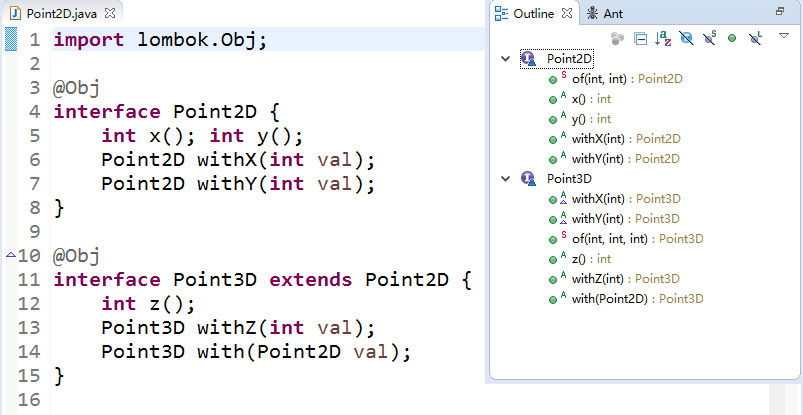
\includegraphics[width=5in]{screenshot.png}
\caption{Screenshot.}\label{screenshot_png}
\end{figure}

\haoyuan{I tried to understand the current algorithm, and did more experiments in eclipse.
Now I borrow some ideas from the current version, and give a new version of the algorithm in text. See below.

(1) I guess the function \textsf{tops} is not necessary. The first step is still
\[\textsf{mbody}(m,C_i)\in\overline{meth}\textrm{ (excluding \textbf{static} methods)}\]

(2) Assume the context is ``interface $C_0$ extends $\overline{C}$ \{$meth'$;...\}''. First handle
\[\textsf{override}(meth',\overline{meth}) \eqno{(*)}\]

(3) If $meth'\ne\none$, $(*)$ returns $meth'$ if
\[\forall meth\in\overline{meth},meth'\subtype meth\]
even if there are conflicts in $\overline{meth}$.

(4) If $meth'=\none$, we need to figure out
\[\textsf{mostSpecific}(\overline{meth})\]
and it should be the one that ``overrides'' all the others in $\overline{meth}$. It means we should not only deal with the return types of methods, but also look into the subtyping relation of interfaces. But for abstract methods, only return types are taken into consideration.
}
\end{comment}

%\text{\yanlin{shouldn't mostSpecific be: $\forall \method' \in \methods : \method \subtype
%  \method'$ ?}}

%(2) If $body_1.\textsf{returnType}=body_2.\textsf{returnType}$, \textsf{shadow} tends to return a default method. If both $body_1$ and $body_2$ are default methods, \textsf{shadow} throws an error.
%\begin{equation*}
%\begin{array}{ll}
%\textsf{shadow}(body_1, body_2)=\textsf{ERROR} & \textsf{if }body_1.\textsf{modifier}=body_2.\textsf{modifier}=\textbf{default}\\
%\textsf{shadow}(body_1, body_2)=body_1 \hspace{.1in} & \textsf{if }body_1.\textsf{modifier}=\textbf{default} \\
%\textsf{shadow}(body_1, body_2)=body_2 \hspace{.1in} & \textsf{if }body_2.\textsf{modifier}=\textbf{default} \\
%\textsf{shadow}(body_1, body_2)=body_1\textsf{ (or }body_2\textsf{)} \hspace{.1in} & \textsf{otherwise}
%\end{array}
%\end{equation*}
%
%(3) If $body_1.\textsf{returnType}<:body_2.\textsf{returnType}$, \textsf{shadow} tends to choose the one with the subtype (namely $body_1$), but only when both methods are abstract, otherwise it gives an error. The other direction $body_2.\textsf{returnType}<:body_1.\textsf{returnType}$ follows the same rule. It also gives an error if there is no subtyping relationship between two return types.
%\begin{equation*}
%\begin{array}{ll}
%\textsf{shadow}(body_1, body_2)=body_1 & \textsf{if }body_1.\textsf{modifier}=body_2.\textsf{modifier}=\emptyset\\
%& \textsf{and }body_1.\textsf{returnType}<:body_2.\textsf{returnType}\\
%\textsf{shadow}(body_1, body_2)=body_2 & \textsf{if }body_1.\textsf{modifier}=body_2.\textsf{modifier}=\emptyset\\
%& \textsf{and }body_2.\textsf{returnType}<:body_1.\textsf{returnType}\\
%\textsf{shadow}(body_1, body_2)=\textsf{ERROR} \hspace{.1in} & \textsf{otherwise}
%\end{array}
%\end{equation*}

%\subsubsection{Auxiliary function: \textsf{replace}}
%
%The \textsf{replace} function takes two same methods (with the same name and types of arguments), and gives the result of the first method overriding the second one.
%
%\begin{equation*}
%\begin{array}{ll}
%\textsf{replace}(body_1, body_2)=body_1 & \textsf{if }body_2=\emptyset\\
%\textsf{replace}(body_1, body_2)=body_2 & \textsf{if }body_1=\emptyset\\
%\textsf{replace}(body_1, body_2)=body_1 & \textsf{if }body_1.\textsf{returnType}<:body_2.\textsf{returnType}\\
%\textsf{replace}(body_1, body_2)=\textsf{ERROR} \hspace{.1in} & \textsf{otherwise}
%\end{array}
%\end{equation*}
